%!TEX root = FreeRtos ARM uController.tex
\subsection{Zielsystem STM32F4 (ARM Cortex M4)}
\label{sec:Zielsysteme}
Der STM32F4 ist ein von STMicroelectronics entwickelter 32 Bit $\mu$Controller, basierend auf einem ARM Cortex M4 Kern. Der STM32F4 arbeitet mit maximal 168 Mhz. \newline
Neben seinen unzähligen Schnittstellen (4x UART, SPI, I2C, Ethernet) bietet der STM32F4 mehrere Energiespar-Modi, die ihn für den Einsatz in energieeffizienten Anwendungen, wie IOT Devices interessant machen. Für die Verwendung von FreeRTOS eignet sich der $\mu$Controller besonders gut, da speziell für diesen $\mu$Controller viele Hardware Funk\-tio\-na\-li\-tät\-en in den FreeRTOS Kernel integriert wurden. Der STM32F4 ist seit 2012 auf dem Markt und erfährt durch eine große Anzahl an Online-Beispielen eine hohe Beliebtheit in der Entwickler-Community. Für den Zugriff auf $\mu$Controller Funktionen stellt STM den Hardware Abstraction Layer (Abbildung \ref{fig:HAL}), kurz HAL, zur Ver\-fü\-gung.      
\begin{figure}[htb!]
	\centering
		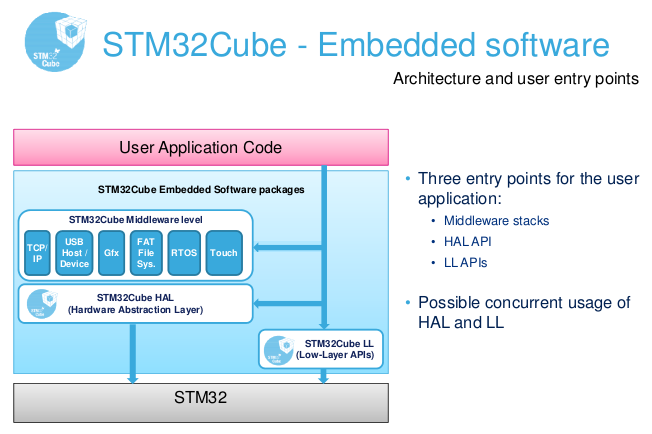
\includegraphics[width=0.4\textwidth]{Pictures/STM32F4/LibraryEntry.png}
	\caption{Aufbau der zur Verfügung stehenden STM Bibliotheken }
	\label{fig:HAL}
\end{figure}
\newline
Der HAL ermöglicht eine einfache Verwendung der Hardware ohne großen Konfigurationsaufwand. Wie spezielle Hardware-Funktionen des STM32F4 durch FreeRTOS genutzt werden, wird in Abschnitt \ref{sec:Low Power Modes} und Abschnitt \ref{sec:Memory Protection} gezeigt.